\documentclass[11pt, oneside]{article}   	% use "amsart" instead of "article" for AMSLaTeX format
\usepackage{geometry}                		% See geometry.pdf to learn the layout options. There are lots.
\geometry{letterpaper}                   		% ... or a4paper or a5paper or ... 
%\geometry{landscape}                		% Activate for for rotated page geometry
%\usepackage[parfill]{parskip}    		% Activate to begin paragraphs with an empty line rather than an indent
\usepackage{graphicx}				% Use pdf, png, jpg, or eps§ with pdflatex; use eps in DVI mode
								% TeX will automatically convert eps --> pdf in pdflatex		
\usepackage{amssymb}
\usepackage{amsmath}
\usepackage{parskip}
\usepackage{color}
\usepackage{hyperref}

\title{Tilted square}
%\author{The Author}
%\section{}
%\subsection*{}
\date{}							% Activate to display a given date or no date

\graphicspath{{/Users/telliott_admin/Dropbox/Tex/png/}}
% \begin{center} 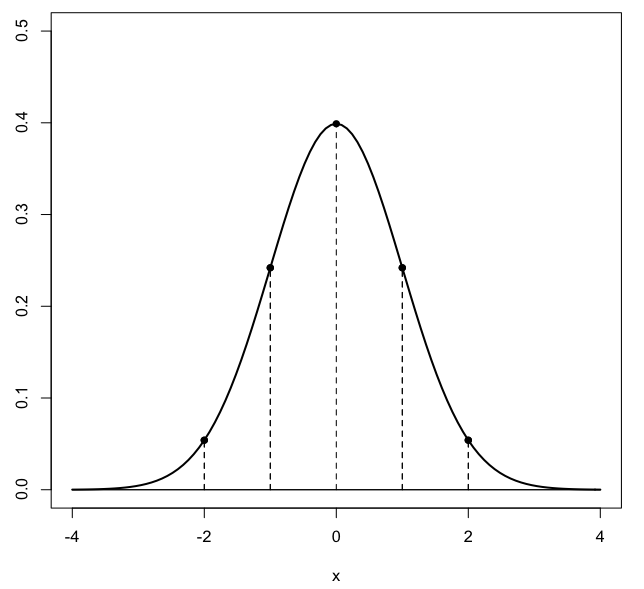
\includegraphics [scale=0.4] {gauss3.png} \end{center}
\begin{document}
\maketitle
\Large
I want to compute the area of the "tilted square" --- in this example, rotated by $45$ degrees with vertices at $(0,0)$, $(1,1)$, $(2,0)$, and $(-1,1)$.  

\begin{center} 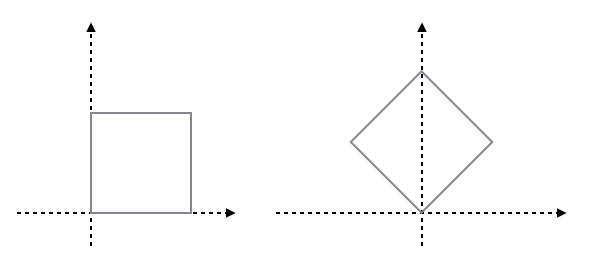
\includegraphics [scale=0.4] {tilted1.png} \end{center}

It is also stretched, note that this is a square with sides of length $\sqrt{2}$ and thus area equal to $2$.

Suppose we integrate first over $y$ and then over $x$.  to the right of the origin, the lower bound is the line $y=x$ and the upper bound is $y = 2-x$.  

To the left of the origin, the lower bound is $y = -x$ and the upper bound is $y = 2+x$.  But we can use symmetry and just compute the part for $x \ge 0$, then double it to get the final answer.  

As we said, we integrate first over $y$:

\[ A = \int_0^1 \int_{y=x}^{y=2-x} \ dy \ dx \]
The inner integral is
\[ \int_{x}^{2-x} \ dy = y \ \bigg |_{x}^{2-x} \]
\[ = 2 - x - x = 2 - 2x = 2 (1-x) \]
and the outer integral is then
\[ = 2 \int_{0}^{1} 1-x \ dx \]
\[ = 2 \ [ \ x - \frac{x^2}{2} \ ] \ \bigg |_0^1 = 2 \ \frac{1}{2} = 1 \]

For the whole area we have another factor of $2$ and the total is thus $2$.  This matches what we get from basic geometry.

Now, let's compute the average value of $y$ over the region.  We need to get what is called the \emph{moment} of $y$:
\[ \int \int y \ dy \ dx \]
We will then divide by the area to get the average value.  This is equivalent to the single variable case:
\[ \bar{x} = \frac{\int_a^b x \ dx }{b - a} \]

The integral is:
\[ \int_0^1 \int_{y=x}^{y=2-x} y \ dy \ dx \]
The inner integral is 
\[ \frac{y^2}{2} \ \bigg |_{x}^{2-x} = \frac{1}{2} (4 - 4x + x^2 - x^2) = 2(1 - x) \]
which is the same as before.  The outer integral is also the same.
\[ 2 \int_0^1 1 - x \ dx = 2 \ [ \ (x-\frac{x^2}{2} ) \ \bigg |_0^1 \ ] = 1 \]
And then $\bar{y}$ is equal to this value divided by the area of the region, which is also equal to $1$, leaving the answer as just $1$.  We can see from the symmetry of the problem that this must be correct.  Moving along the $x$-axis (for each value of $x$), we're looking at a line where for each value of $y = 1 + \delta$ above the value $y=1$ there is another value $y = 1 - \delta$ below.  So the average value of $y$ is indeed just $1$.

For practice, suppose we reverse the order and compute the $x$ integral first.  

Because the equation relating the upper bound of $x$ as a function of $y$ changes at $y=1$ we split the integral into two parts:
\[ \int_0^1 \int_{x=0}^{x=y} \ dx \ dy  + \int_1^2 \int_{x=0}^{x=2-y} \ dx \ dy \]
The inner integral is just $y$ for the first term and $2-y$ for the second (but remember the bounds are different).  So we obtain
\[ = \int_0^1 y \ dy + \int_1^2 (2-y) \ dy \]
\[ = \frac{y^2}{2} \ \bigg |_0^1 + 2y \ \bigg |_1^2 - \frac{y^2}{2} \ \bigg |_1^2 \]
\[ = \frac{1}{2} + 2 - \frac{3}{2} = 1 \]
This matches what we got by computing the $y$-integral first, as it must.

Now we compute the average value of the function $f(x,y) = y$ over the same region.  
\[ \int_0^1 \int_{x=0}^{x=y} y \ dx \ dy  + \int_1^2 \int_{x=0}^{x=2-y} y \ dx \ dy \]
The inner integrals are
\[ xy \ \bigg |_0^y = y^2 \]
and
\[  xy \ \bigg |_0^{2-y} = y(2-y) \]
The outer integral is 
\[ \int_0^1 y^2 \ dy + \int_1^2 2y \ dy - \int_1^2 y^2 \ dy \]
\[ = \frac{y^3}{3} \ \bigg |_0^1 + y^2 \ \bigg |_1^2 - \frac{y^3}{3} \ \bigg |_1^2 \]
\[ = \frac{1}{3} + 3 - \ [ \ \frac{8}{3} - \frac{1}{3} \ ] = 1 \]

A different way to do the area problem to use a change of variable, which simplifies that problem quite a bit, at the expense of changing the area element.

We would like to tilt the square back to horizontal so that
\[ (0,0) \rightarrow (0,0) \]
\[ (1,1) \rightarrow (1,0) \]
\[ (0,2) \rightarrow (1,1) \]
\[ (-1,1) \rightarrow (0,1) \]
By guessing I find that the transformation that does this is:
\[ u = \frac{1}{2} (x+y) \]
\[ v =  \frac{1}{2} (y-x) \]
Since this is a linear transformation and it gives the correct answers for the vertices,   it works for all interior points as well.

For the area problem, the area of the re-tilted square is equal to $1$ in the $u,v$-coordinate system.

That's a good reason to do this transformation.  We get to the correct value for the area in $x,y$-coordinates by remembering that the area elements are not the same.  That is
\[ dx \ dy \ne du \ dv \]
The scaling factor is obtained computing the absolute value of the determinant of the Jacobian (a mouthful for sure), but it is just

\[ 
J = 
\begin{vmatrix}
u_x  &  u_y \\
v_x  &  v_y 
\end{vmatrix} 
\
\begin{vmatrix}
\ 1/2  &  1/2 \\
- 1/2   & 1/2
\end{vmatrix} 
= \frac{1}{2}
\]
So the area elements are related by
\[  du \ dx = J  \ dx \ dy \]
The area as computed under the transformation is one-half the area in the standard coordinate system.  We obtained $1$ as the answer in $u,v$-coordinates so we multiply by $2$ and obtain the answer for $x,y$-coordinates, which matches what we had before.

We can also compute the average value of $y$, but first we need an expression for $y$ in terms of $u$ and $v$.  I add the above equations to obtain:

\[ y = u + v \]
So the integral we must compute for the average value is 
\[ \frac{1}{2} \iint y \ dy \ dx = \iint (u + v) \ du \ dv \]
The limits are easy
\[ = \int_0^1 \int_0^1 u + v \ du \ dv \]
The inner integral is
\[ \int u + v \ du = \frac{u^2}{2} + uv \ \bigg |_0^1 = \frac{1}{2} + v \]
The outer integral is then
\[ \int_0^1  \frac{1}{2} + v  \ dv = \frac{1}{2} + \frac{1}{2} = 1 \]
remembering the factor of $1/2$, the final answer is $1/2$.  This, divided by the area is the average value of $y$ in the $u,v$-coordinate system.

So how does this stack up against the original answer for $\bar{y}$ and what the geometry tells us?

Still working on this, but my feeling about it is that we are looking at $y$ as we slide from $(-1,1) \rightarrow (1,1)$  in $x,y$ coordinates which is the same as sliding from $(1,0)$ to $(0,1)$ in $u,v$-coordinates. 

Since we have $y = 1 \rightarrow 0$ linearly with $x$, the answer is obviously correct.

The real advantage of the transformation approach is that we can tilt to any angle.  

\begin{center} 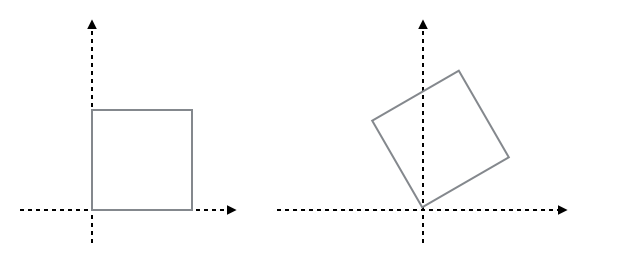
\includegraphics [scale=0.4] {tilted2.png} \end{center}
Recall that if we turn a vector by an angle $\phi$ counter-clockwise, the equations are
\[ u = x \cos \phi - y \sin \phi \]
\[ v = x \sin \phi + y \cos \phi \]

It is easy to get mixed up and do the calculations with the wrong sign.  When we \emph{start} with the tilted square and then transform it to the standard orientation we can think of it as either a CW orientation of the points, or a CCW rotation of the coordinates.  In any event, the sign of sine in the equations is the opposite of what we have above.

\[ u = x \cos \phi + y \sin \phi \]
\[ v = -x \sin \phi + y \cos \phi \]

We check this by asking about $\phi = \pi/2$.  Then we have
\[ u = y \]
\[ v = -x \]
The vectors or points:
\[ (0,1) \rightarrow (1,0) \]
\[ (-1,0) \rightarrow (0,1) \]
which is correct for a clockwise turn of $90$ degrees.  Since the equations work for unit vectors along the $x$ and $y$-axes, they will work for any vector or any point.

In contrast to what we did above, this is not a stretching transformation.
\[ 
J = 
\begin{vmatrix}
u_x  &  u_y \\
v_x  &  v_y 
\end{vmatrix} 
\
\begin{vmatrix}
-\sin \phi  &  \cos \phi \\
\ \ -\cos \phi  & - \sin \phi
\end{vmatrix} 
= \sin^2 \phi - (- \cos^2 \phi) = 1 
\]

The limits are great:  $0 \rightarrow 1$.  The area of the square is
\[ \frac{1}{J} \int_0^1 \int_0^1 \ du \ dv = 1 \]

To find the moment of $y$ we can go back to our equations
\[ u = x \cos \phi + y \sin \phi \]
\[ v = -x \sin \phi + y \cos \phi \]
To get, say, $y$ as a function of $u$ and $v$ we can isolate $y$ as follows
\[ u \sin \phi = x \sin \phi \cos \phi + y \sin^2 \phi \]
\[ v \cos \phi = x \sin \phi \cos \phi + y \cos^2 \phi \]
Adding:
\[ y = u \sin \phi + v \cos \phi \]
or we can remember to just switch the sign of the sines when we switch letters in the original equation:
\[ x = u \cos \phi - v \sin \phi \]
\[ y = u \sin \phi + v \cos \phi \]
Hence
\[ \iint y \ dA = \int \int u \sin \phi + v \cos \phi \ du \ dv \]
where $\phi$ is a constant.

The inner integral is:
\[ \int_0^1 (u \sin \phi + v \cos \phi ) \ du = \frac{1}{2} \sin \phi + \cos \phi \ v \]
and the outer integral is
\[ \int_0^1  (\frac{1}{2} \sin \phi + \cos \phi \ v)  \ dv \]
\[ = \frac{1}{2} (\cos \phi + \sin \phi) \]

If we do the integrals for $x$ as well then we will have:
\[ \bar{x} =  \frac{1}{2} (\cos \phi - \sin \phi) \]
\[ \bar{y} =  \frac{1}{2} (\cos \phi + \sin \phi) \]

The average value of $x$ and $y$ are these values divided by the area (which was equal to $1$).

We can see that we have our signs correct here.  If we tilt counter-clockwise, then the average value of $x$ passes through zero and goes negative, which the average value of $y$ will stay positive, reaching a maximum at $\phi = \pi/4$.

Notice that if there is no turning ($\phi = 0$) or if $\phi = \pi/2$, then the average value $\bar{x} = \bar{y} = 1/2$, as expected.  

If $\phi = \pi/4$ then $ \bar{x} =0$, as expected, and $\bar{y} = 1/\sqrt{2} \approx 0.7$.

And if $\phi = \pi/2$ then $\bar{x} = - 1/2$ and $\bar{y} = 1/2$.

If we differentiate and set the derivative equal to zero, the maximum $\bar{y}$ is:
\[ \frac{d}{d \phi} \bar{y} =  \frac{1}{2} (- \sin \phi + \cos \phi) = 0 \]
\[ \sin \phi = \cos \phi \]
\[ \phi = \frac{\pi}{4} \]

\end{document}  